\section{Containerization}
We have containerized our project using \textbf{Docker}. Docker is a platform that allows us to develop, ship, and run applications in containers.
Both Django (backend) and Nuxt (frontend) are running as a docker container.
We have written dockerfiles individually for both the backend and the frontend, and also used two public images of Postgresql and Redis.
The docker files are located in each of the directories of the backend and the frontend.
We have also used docker-compose to run all the containers together, which is a tool for defining and running multi-container Docker applications.

Figure \ref{fig:architecture} shows the top level architecture of the project.

\begin{figure}[htbp]
    \centering
    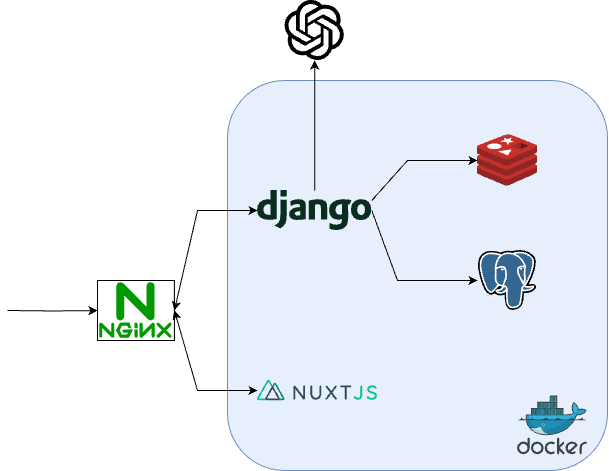
\includegraphics[width=0.4\linewidth]{img/infra.png}
    \caption{Architecture of the project}
    \label{fig:architecture}
\end{figure}

\section{Environments}
We used to seperate environments for development and other for production, each of these environments have their own configuration files.
The files are located in the `deploy` directory.


\section{Server}
Since we already had the dockerized version of our project working on our local machines, we decided to deploy our project on a simple virtual private server (VPS) using \textbf{DigitalOcean}.
We have securely configured the VPS to build and run the docker containers.
We are using Nginx as a reverse proxy to route the incoming requests to the appropriate internal container, and also handle the SSL certificates.
The domain we have used is `\url{the-hive.space}`, which we have purchased for use exclusively for this project.

\section{Continuous Deployment}
Using Github Actions, we have setup a continuous deployment pipeline that builds and deploys the project to the VPS whenever a new commit is pushed to the main branch.
